\documentclass[border=8pt]{standalone}
\usepackage[T1]{fontenc}
\usepackage{mathptmx}
\usepackage{tikz}
\usetikzlibrary{arrows.meta,positioning,fit,calc,shapes.geometric,shapes.misc,shapes.multipart,backgrounds}
\tikzset{
  arr/.style={-{Stealth[length=2.4mm,width=1.8mm]},line width=0.6pt},
  box/.style={draw,line width=0.6pt,align=center,rounded corners=2pt},
}

\begin{document}
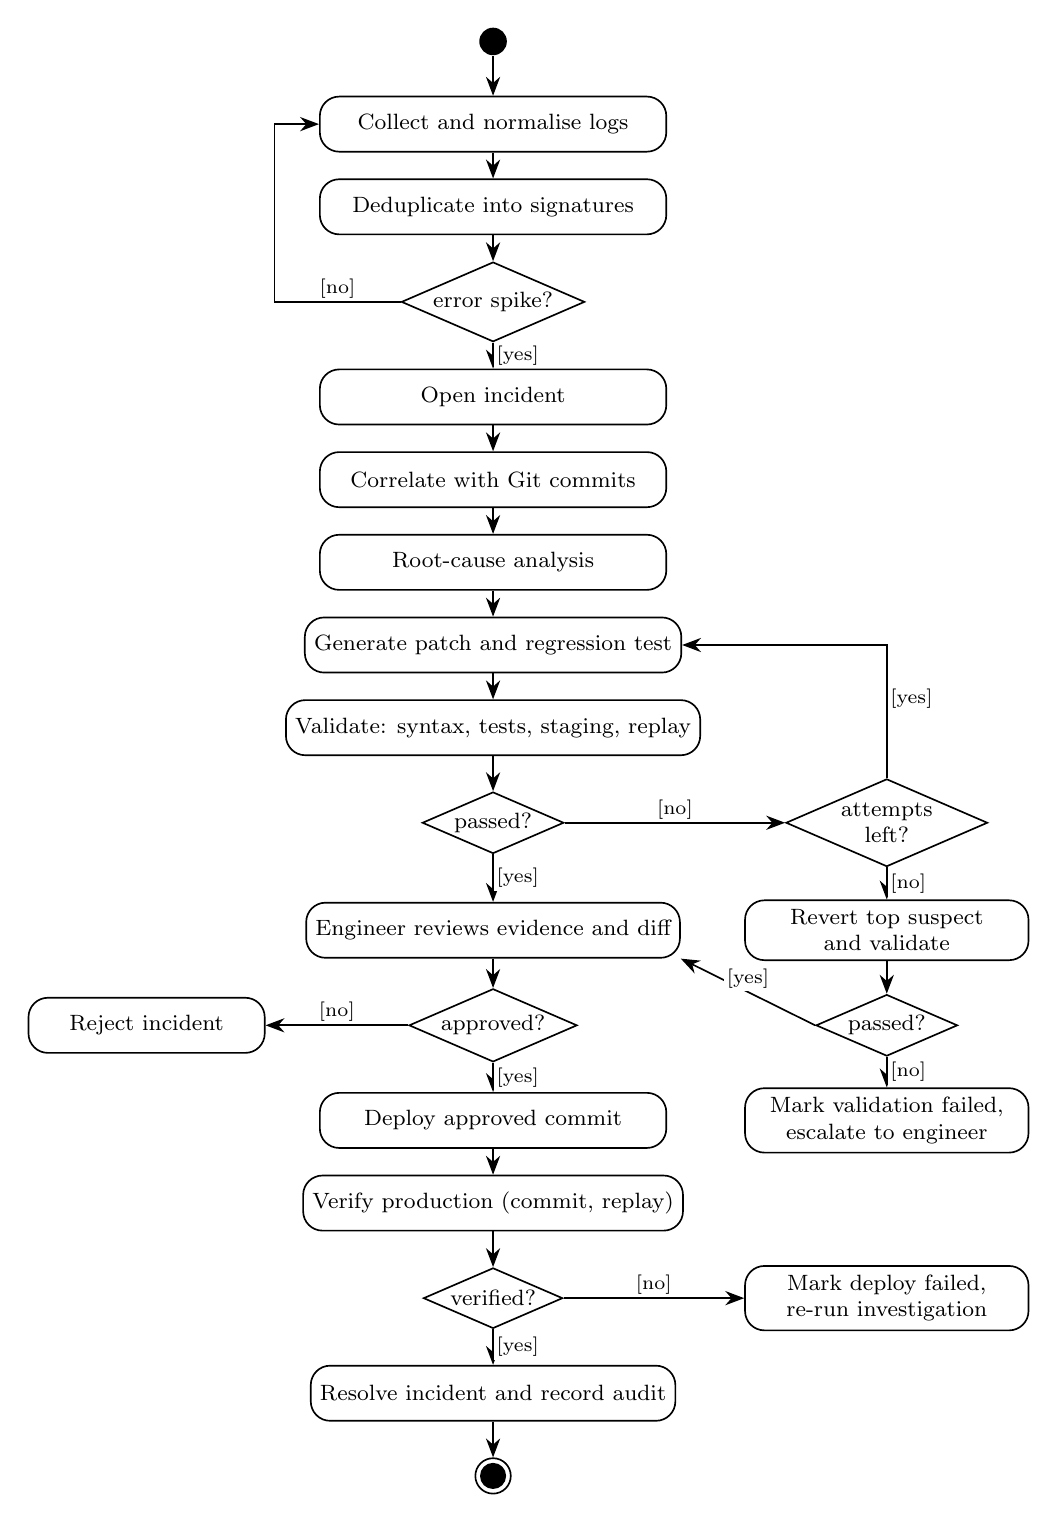
\begin{tikzpicture}[font=\footnotesize,
  a/.style={draw, rounded corners=7pt, line width=0.6pt, minimum width=4.4cm, minimum height=0.7cm, align=center},
  d/.style={draw, diamond, aspect=2.3, line width=0.6pt, inner sep=1pt, align=center},
  g/.style={font=\scriptsize, inner sep=1pt, fill=white}]
\def\s{1.05}
\node[circle, fill=black, minimum size=0.35cm] (st) at (0,0) {};
\node[a] (a1) at (0,-1*\s) {Collect and normalise logs};
\node[a] (a2) at (0,-2*\s) {Deduplicate into signatures};
\node[d] (d1) at (0,-3.15*\s) {error spike?};
\node[a] (a3) at (0,-4.3*\s) {Open incident};
\node[a] (a4) at (0,-5.3*\s) {Correlate with Git commits};
\node[a] (a5) at (0,-6.3*\s) {Root-cause analysis};
\node[a] (a6) at (0,-7.3*\s) {Generate patch and regression test};
\node[a] (a7) at (0,-8.3*\s) {Validate: syntax, tests, staging, replay};
\node[d] (d2) at (0,-9.45*\s) {passed?};
\node[a] (a9) at (0,-10.75*\s) {Engineer reviews evidence and diff};
\node[d] (d5) at (0,-11.9*\s) {approved?};
\node[a] (a12) at (0,-13.05*\s) {Deploy approved commit};
\node[a] (a13) at (0,-14.05*\s) {Verify production (commit, replay)};
\node[d] (d6) at (0,-15.2*\s) {verified?};
\node[a] (a15) at (0,-16.35*\s) {Resolve incident and record audit};
\node[circle, draw, line width=0.6pt, minimum size=0.45cm] (fin) at (0,-17.35*\s) {}; \node[circle, fill=black, minimum size=0.28cm] at (fin) {};
\node[d] (d3) at (5.0,-9.45*\s) {attempts\\ left?};
\node[a, minimum width=3.6cm] (a8) at (5.0,-10.75*\s) {Revert top suspect\\ and validate};
\node[d] (d4) at (5.0,-11.9*\s) {passed?};
\node[a, minimum width=3.6cm] (a10) at (5.0,-13.05*\s) {Mark validation failed,\\ escalate to engineer};
\node[a, minimum width=3.0cm] (a11) at (-4.4,-11.9*\s) {Reject incident};
\node[a, minimum width=3.6cm] (a14) at (5.0,-15.2*\s) {Mark deploy failed,\\ re-run investigation};
\foreach \u/\v in {st/a1,a1/a2,a2/d1,a3/a4,a4/a5,a5/a6,a6/a7,a7/d2,a9/d5,a12/a13,a13/d6,a15/fin}{\draw[arr] (\u)--(\v);}
\draw[arr] (d1) -- node[g, right] {[yes]} (a3);
\draw[arr] (d1.west) -- node[g, above] {[no]} ++(-1.6,0) |- (a1.west);
\draw[arr] (d2) -- node[g, right] {[yes]} (a9);
\draw[arr] (d2.east) -- node[g, above] {[no]} (d3.west);
\draw[arr] (d3.north) |- node[g, pos=0.3, right] {[yes]} (a6.east);
\draw[arr] (d3) -- node[g, right] {[no]} (a8);
\draw[arr] (a8) -- (d4);
\draw[arr] (d4.west) -- node[g, above] {[yes]} (a9.south east);
\draw[arr] (d4) -- node[g, right] {[no]} (a10);
\draw[arr] (d5) -- node[g, right] {[yes]} (a12);
\draw[arr] (d5.west) -- node[g, above] {[no]} (a11.east);
\draw[arr] (d6) -- node[g, right] {[yes]} (a15);
\draw[arr] (d6.east) -- node[g, above] {[no]} (a14.west);
\end{tikzpicture}
\end{document}
